\documentclass[twoside]{book}

% Packages required by doxygen
\usepackage{fixltx2e}
\usepackage{calc}
\usepackage{doxygen}
\usepackage[export]{adjustbox} % also loads graphicx
\usepackage{graphicx}
\usepackage[utf8]{inputenc}
\usepackage{makeidx}
\usepackage{multicol}
\usepackage{multirow}
\PassOptionsToPackage{warn}{textcomp}
\usepackage{textcomp}
\usepackage[nointegrals]{wasysym}
\usepackage[table]{xcolor}

% Font selection
\usepackage[T1]{fontenc}
\usepackage[scaled=.90]{helvet}
\usepackage{courier}
\usepackage{amssymb}
\usepackage{sectsty}
\renewcommand{\familydefault}{\sfdefault}
\allsectionsfont{%
  \fontseries{bc}\selectfont%
  \color{darkgray}%
}
\renewcommand{\DoxyLabelFont}{%
  \fontseries{bc}\selectfont%
  \color{darkgray}%
}
\newcommand{\+}{\discretionary{\mbox{\scriptsize$\hookleftarrow$}}{}{}}

% Page & text layout
\usepackage{geometry}
\geometry{%
  a4paper,%
  top=2.5cm,%
  bottom=2.5cm,%
  left=2.5cm,%
  right=2.5cm%
}
\tolerance=750
\hfuzz=15pt
\hbadness=750
\setlength{\emergencystretch}{15pt}
\setlength{\parindent}{0cm}
\setlength{\parskip}{0.2cm}
\makeatletter
\renewcommand{\paragraph}{%
  \@startsection{paragraph}{4}{0ex}{-1.0ex}{1.0ex}{%
    \normalfont\normalsize\bfseries\SS@parafont%
  }%
}
\renewcommand{\subparagraph}{%
  \@startsection{subparagraph}{5}{0ex}{-1.0ex}{1.0ex}{%
    \normalfont\normalsize\bfseries\SS@subparafont%
  }%
}
\makeatother

% Headers & footers
\usepackage{fancyhdr}
\pagestyle{fancyplain}
\fancyhead[LE]{\fancyplain{}{\bfseries\thepage}}
\fancyhead[CE]{\fancyplain{}{}}
\fancyhead[RE]{\fancyplain{}{\bfseries\leftmark}}
\fancyhead[LO]{\fancyplain{}{\bfseries\rightmark}}
\fancyhead[CO]{\fancyplain{}{}}
\fancyhead[RO]{\fancyplain{}{\bfseries\thepage}}
\fancyfoot[LE]{\fancyplain{}{}}
\fancyfoot[CE]{\fancyplain{}{}}
\fancyfoot[RE]{\fancyplain{}{\bfseries\scriptsize Generated by Doxygen }}
\fancyfoot[LO]{\fancyplain{}{\bfseries\scriptsize Generated by Doxygen }}
\fancyfoot[CO]{\fancyplain{}{}}
\fancyfoot[RO]{\fancyplain{}{}}
\renewcommand{\footrulewidth}{0.4pt}
\renewcommand{\chaptermark}[1]{%
  \markboth{#1}{}%
}
\renewcommand{\sectionmark}[1]{%
  \markright{\thesection\ #1}%
}

% Indices & bibliography
\usepackage{natbib}
\usepackage[titles]{tocloft}
\setcounter{tocdepth}{3}
\setcounter{secnumdepth}{5}
\makeindex

% Hyperlinks (required, but should be loaded last)
\usepackage{ifpdf}
\ifpdf
  \usepackage[pdftex,pagebackref=true]{hyperref}
\else
  \usepackage[ps2pdf,pagebackref=true]{hyperref}
\fi
\hypersetup{%
  colorlinks=true,%
  linkcolor=blue,%
  citecolor=blue,%
  unicode%
}

% Custom commands
\newcommand{\clearemptydoublepage}{%
  \newpage{\pagestyle{empty}\cleardoublepage}%
}


%===== C O N T E N T S =====

\begin{document}

% Titlepage & ToC
\hypersetup{pageanchor=false,
             bookmarks=true,
             bookmarksnumbered=true,
             pdfencoding=unicode
            }
\pagenumbering{roman}
\begin{titlepage}
\vspace*{7cm}
\begin{center}%
{\Large Block\+World (G\+L\+E\+X) }\\
\vspace*{1cm}
{\large Generated by Doxygen 1.8.10}\\
\end{center}
\end{titlepage}
\clearemptydoublepage
\tableofcontents
\clearemptydoublepage
\pagenumbering{arabic}
\hypersetup{pageanchor=true}

%--- Begin generated contents ---
\chapter{Hierarchical Index}
\section{Class Hierarchy}
This inheritance list is sorted roughly, but not completely, alphabetically\+:\begin{DoxyCompactList}
\item \contentsline{section}{Camera}{\pageref{classCamera}}{}
\item \contentsline{section}{Game\+Asset}{\pageref{classGameAsset}}{}
\begin{DoxyCompactList}
\item \contentsline{section}{Cube\+Asset}{\pageref{classCubeAsset}}{}
\item \contentsline{section}{Ground\+Asset}{\pageref{classGroundAsset}}{}
\item \contentsline{section}{Star\+Asset}{\pageref{classStarAsset}}{}
\end{DoxyCompactList}
\item \contentsline{section}{Game\+Asset\+Manager}{\pageref{classGameAssetManager}}{}
\item \contentsline{section}{Game\+World}{\pageref{classGameWorld}}{}
\item \contentsline{section}{S\+D\+L\+Window\+Deleter}{\pageref{structSDLWindowDeleter}}{}
\end{DoxyCompactList}

\chapter{Class Index}
\section{Class List}
Here are the classes, structs, unions and interfaces with brief descriptions\+:\begin{DoxyCompactList}
\item\contentsline{section}{\hyperlink{classApp}{App} }{\pageref{classApp}}{}
\item\contentsline{section}{\hyperlink{classBoundingBox}{Bounding\+Box} }{\pageref{classBoundingBox}}{}
\item\contentsline{section}{\hyperlink{classCamera}{Camera} }{\pageref{classCamera}}{}
\item\contentsline{section}{\hyperlink{classColourManager}{Colour\+Manager} }{\pageref{classColourManager}}{}
\item\contentsline{section}{\hyperlink{classCubeAsset}{Cube\+Asset} }{\pageref{classCubeAsset}}{}
\item\contentsline{section}{\hyperlink{classDiamondAsset}{Diamond\+Asset} }{\pageref{classDiamondAsset}}{}
\item\contentsline{section}{\hyperlink{classGameAsset}{Game\+Asset} }{\pageref{classGameAsset}}{}
\item\contentsline{section}{\hyperlink{classGameAssetManager}{Game\+Asset\+Manager} }{\pageref{classGameAssetManager}}{}
\item\contentsline{section}{\hyperlink{classGameWorld}{Game\+World} }{\pageref{classGameWorld}}{}
\item\contentsline{section}{\hyperlink{classPythonBindings}{Python\+Bindings} }{\pageref{classPythonBindings}}{}
\item\contentsline{section}{\hyperlink{structSDLWindowDeleter}{S\+D\+L\+Window\+Deleter} }{\pageref{structSDLWindowDeleter}}{}
\item\contentsline{section}{\hyperlink{classStarAsset}{Star\+Asset} }{\pageref{classStarAsset}}{}
\end{DoxyCompactList}

\chapter{Class Documentation}
\hypertarget{classApp}{}\section{App Class Reference}
\label{classApp}\index{App@{App}}
\subsection*{Public Member Functions}
\begin{DoxyCompactItemize}
\item 
std\+::shared\+\_\+ptr$<$ S\+D\+L\+\_\+\+Window $>$ \hyperlink{classApp_ab4c0c84fff9897a7d8bc689de35a33d8}{Init\+World} ()
\item 
void \hyperlink{classApp_aeafb49d25856793f0f7367d8b8a8b6c4}{Draw} (const std\+::shared\+\_\+ptr$<$ S\+D\+L\+\_\+\+Window $>$ \&window, const std\+::shared\+\_\+ptr$<$ \hyperlink{classGameWorld}{Game\+World} $>$ \&game\+\_\+world)
\item 
void \hyperlink{classApp_a78d24016da98422fabb55b10dbfe3d72}{Run} ()
\item 
void \hyperlink{classApp_acf46a5740892f0d89ee5b47da2bf99ff}{Handle\+Input} (const std\+::shared\+\_\+ptr$<$ \hyperlink{classGameWorld}{Game\+World} $>$ \&game\+\_\+world)
\end{DoxyCompactItemize}


\subsection{Member Function Documentation}
\hypertarget{classApp_aeafb49d25856793f0f7367d8b8a8b6c4}{}\index{App@{App}!Draw@{Draw}}
\index{Draw@{Draw}!App@{App}}
\subsubsection[{Draw(const std\+::shared\+\_\+ptr$<$ S\+D\+L\+\_\+\+Window $>$ \&window, const std\+::shared\+\_\+ptr$<$ Game\+World $>$ \&game\+\_\+world)}]{\setlength{\rightskip}{0pt plus 5cm}void App\+::\+Draw (
\begin{DoxyParamCaption}
\item[{const std\+::shared\+\_\+ptr$<$ S\+D\+L\+\_\+\+Window $>$ \&}]{window, }
\item[{const std\+::shared\+\_\+ptr$<$ {\bf Game\+World} $>$ \&}]{game\+\_\+world}
\end{DoxyParamCaption}
)}\label{classApp_aeafb49d25856793f0f7367d8b8a8b6c4}
Draws the colour and calls to \hyperlink{classGameWorld}{Game\+World} for Drawing \hypertarget{classApp_acf46a5740892f0d89ee5b47da2bf99ff}{}\index{App@{App}!Handle\+Input@{Handle\+Input}}
\index{Handle\+Input@{Handle\+Input}!App@{App}}
\subsubsection[{Handle\+Input(const std\+::shared\+\_\+ptr$<$ Game\+World $>$ \&game\+\_\+world)}]{\setlength{\rightskip}{0pt plus 5cm}void App\+::\+Handle\+Input (
\begin{DoxyParamCaption}
\item[{const std\+::shared\+\_\+ptr$<$ {\bf Game\+World} $>$ \&}]{game\+\_\+world}
\end{DoxyParamCaption}
)}\label{classApp_acf46a5740892f0d89ee5b47da2bf99ff}
Handles global input from mouse and keyboard \hypertarget{classApp_ab4c0c84fff9897a7d8bc689de35a33d8}{}\index{App@{App}!Init\+World@{Init\+World}}
\index{Init\+World@{Init\+World}!App@{App}}
\subsubsection[{Init\+World()}]{\setlength{\rightskip}{0pt plus 5cm}std\+::shared\+\_\+ptr$<$ S\+D\+L\+\_\+\+Window $>$ App\+::\+Init\+World (
\begin{DoxyParamCaption}
{}
\end{DoxyParamCaption}
)}\label{classApp_ab4c0c84fff9897a7d8bc689de35a33d8}
Initialises the S\+D\+L\+\_\+\+Window and Open\+G\+L 3.\+0 \hypertarget{classApp_a78d24016da98422fabb55b10dbfe3d72}{}\index{App@{App}!Run@{Run}}
\index{Run@{Run}!App@{App}}
\subsubsection[{Run()}]{\setlength{\rightskip}{0pt plus 5cm}void App\+::\+Run (
\begin{DoxyParamCaption}
{}
\end{DoxyParamCaption}
)}\label{classApp_a78d24016da98422fabb55b10dbfe3d72}
Starts our game loop, called via Python or Main 

The documentation for this class was generated from the following files\+:\begin{DoxyCompactItemize}
\item 
App.\+h\item 
App.\+cc\end{DoxyCompactItemize}

\hypertarget{classBoundingBox}{}\section{Bounding\+Box Class Reference}
\label{classBoundingBox}\index{Bounding\+Box@{Bounding\+Box}}
\subsection*{Public Member Functions}
\begin{DoxyCompactItemize}
\item 
\hyperlink{classBoundingBox_a85b1b2999c0810fbfcffe0f82f5ef581}{Bounding\+Box} (glm\+::vec3, int, float, glm\+::vec3, glm\+::vec3)
\item 
glm\+::vec3 \hyperlink{classBoundingBox_ae030e99b894d0326307268ec80a046a9}{Get\+Vec3} ()
\item 
glm\+::mat4 \hyperlink{classBoundingBox_ac8214cfca4958127d0bacd263c6008d4}{Get\+Model\+Transformation} ()
\item 
glm\+::vec3 \hyperlink{classBoundingBox_a968169f93442add1db9b5b4ca9e7d358}{Get\+Max\+And\+Min} (int)
\item 
void \hyperlink{classBoundingBox_afb77ba3c0b8ad8862e92f18adba8258e}{Translate} (glm\+::vec3)
\item 
void \hyperlink{classBoundingBox_a47aa793b888dc49037021c707b83d3fb}{Scale} (float)
\item 
void \hyperlink{classBoundingBox_ad94b5e157e468a21ce7a7ade20a74c09}{Rotate} (glm\+::vec3)
\item 
void \hyperlink{classBoundingBox_aed8d9c54c463e21f4bcdd8340e141cfb}{Check\+Collision} (glm\+::vec3, glm\+::vec3, glm\+::vec3, glm\+::vec3)
\item 
void \hyperlink{classBoundingBox_a91f44328bdf42b85a02538e93f50081c}{Set\+Path} (std\+::vector$<$ glm\+::vec3 $>$)
\item 
void \hyperlink{classBoundingBox_a4bda88b17a66734dea30916f048679c6}{Follow\+Path} ()
\end{DoxyCompactItemize}
\subsection*{Public Attributes}
\begin{DoxyCompactItemize}
\item 
\hypertarget{classBoundingBox_a06fd05f65178892ca298446e7c111f3c}{}std\+::vector$<$ glm\+::vec3 $>$ {\bfseries path\+\_\+list}\label{classBoundingBox_a06fd05f65178892ca298446e7c111f3c}

\end{DoxyCompactItemize}


\subsection{Constructor \& Destructor Documentation}
\hypertarget{classBoundingBox_a85b1b2999c0810fbfcffe0f82f5ef581}{}\index{Bounding\+Box@{Bounding\+Box}!Bounding\+Box@{Bounding\+Box}}
\index{Bounding\+Box@{Bounding\+Box}!Bounding\+Box@{Bounding\+Box}}
\subsubsection[{Bounding\+Box(glm\+::vec3, int, float, glm\+::vec3, glm\+::vec3)}]{\setlength{\rightskip}{0pt plus 5cm}Bounding\+Box\+::\+Bounding\+Box (
\begin{DoxyParamCaption}
\item[{glm\+::vec3}]{position, }
\item[{int}]{type, }
\item[{float}]{scale, }
\item[{glm\+::vec3}]{rotation, }
\item[{glm\+::vec3}]{speed}
\end{DoxyParamCaption}
)}\label{classBoundingBox_a85b1b2999c0810fbfcffe0f82f5ef581}
\hyperlink{classBoundingBox}{Bounding\+Box} initialisation 

\subsection{Member Function Documentation}
\hypertarget{classBoundingBox_aed8d9c54c463e21f4bcdd8340e141cfb}{}\index{Bounding\+Box@{Bounding\+Box}!Check\+Collision@{Check\+Collision}}
\index{Check\+Collision@{Check\+Collision}!Bounding\+Box@{Bounding\+Box}}
\subsubsection[{Check\+Collision(glm\+::vec3, glm\+::vec3, glm\+::vec3, glm\+::vec3)}]{\setlength{\rightskip}{0pt plus 5cm}void Bounding\+Box\+::\+Check\+Collision (
\begin{DoxyParamCaption}
\item[{glm\+::vec3}]{bounding\+\_\+box1\+\_\+max, }
\item[{glm\+::vec3}]{bounding\+\_\+box1\+\_\+min, }
\item[{glm\+::vec3}]{bounding\+\_\+box2\+\_\+max, }
\item[{glm\+::vec3}]{bounding\+\_\+box2\+\_\+min}
\end{DoxyParamCaption}
)}\label{classBoundingBox_aed8d9c54c463e21f4bcdd8340e141cfb}
Check if a bounding box has collided with another \hypertarget{classBoundingBox_a4bda88b17a66734dea30916f048679c6}{}\index{Bounding\+Box@{Bounding\+Box}!Follow\+Path@{Follow\+Path}}
\index{Follow\+Path@{Follow\+Path}!Bounding\+Box@{Bounding\+Box}}
\subsubsection[{Follow\+Path()}]{\setlength{\rightskip}{0pt plus 5cm}void Bounding\+Box\+::\+Follow\+Path (
\begin{DoxyParamCaption}
{}
\end{DoxyParamCaption}
)}\label{classBoundingBox_a4bda88b17a66734dea30916f048679c6}
Follow Path coordiantes \hypertarget{classBoundingBox_a968169f93442add1db9b5b4ca9e7d358}{}\index{Bounding\+Box@{Bounding\+Box}!Get\+Max\+And\+Min@{Get\+Max\+And\+Min}}
\index{Get\+Max\+And\+Min@{Get\+Max\+And\+Min}!Bounding\+Box@{Bounding\+Box}}
\subsubsection[{Get\+Max\+And\+Min(int)}]{\setlength{\rightskip}{0pt plus 5cm}glm\+::vec3 Bounding\+Box\+::\+Get\+Max\+And\+Min (
\begin{DoxyParamCaption}
\item[{int}]{type}
\end{DoxyParamCaption}
)}\label{classBoundingBox_a968169f93442add1db9b5b4ca9e7d358}
Return the max and minimum bounds \hypertarget{classBoundingBox_ac8214cfca4958127d0bacd263c6008d4}{}\index{Bounding\+Box@{Bounding\+Box}!Get\+Model\+Transformation@{Get\+Model\+Transformation}}
\index{Get\+Model\+Transformation@{Get\+Model\+Transformation}!Bounding\+Box@{Bounding\+Box}}
\subsubsection[{Get\+Model\+Transformation()}]{\setlength{\rightskip}{0pt plus 5cm}glm\+::mat4 Bounding\+Box\+::\+Get\+Model\+Transformation (
\begin{DoxyParamCaption}
{}
\end{DoxyParamCaption}
)}\label{classBoundingBox_ac8214cfca4958127d0bacd263c6008d4}
Get the model translformation based on asset type \hypertarget{classBoundingBox_ae030e99b894d0326307268ec80a046a9}{}\index{Bounding\+Box@{Bounding\+Box}!Get\+Vec3@{Get\+Vec3}}
\index{Get\+Vec3@{Get\+Vec3}!Bounding\+Box@{Bounding\+Box}}
\subsubsection[{Get\+Vec3()}]{\setlength{\rightskip}{0pt plus 5cm}glm\+::vec3 Bounding\+Box\+::\+Get\+Vec3 (
\begin{DoxyParamCaption}
{}
\end{DoxyParamCaption}
)}\label{classBoundingBox_ae030e99b894d0326307268ec80a046a9}
Get vec3 for bbox \hypertarget{classBoundingBox_ad94b5e157e468a21ce7a7ade20a74c09}{}\index{Bounding\+Box@{Bounding\+Box}!Rotate@{Rotate}}
\index{Rotate@{Rotate}!Bounding\+Box@{Bounding\+Box}}
\subsubsection[{Rotate(glm\+::vec3)}]{\setlength{\rightskip}{0pt plus 5cm}void Bounding\+Box\+::\+Rotate (
\begin{DoxyParamCaption}
\item[{glm\+::vec3}]{rotate\+\_\+speed}
\end{DoxyParamCaption}
)}\label{classBoundingBox_ad94b5e157e468a21ce7a7ade20a74c09}
Used to rotate by a certain speed \hypertarget{classBoundingBox_a47aa793b888dc49037021c707b83d3fb}{}\index{Bounding\+Box@{Bounding\+Box}!Scale@{Scale}}
\index{Scale@{Scale}!Bounding\+Box@{Bounding\+Box}}
\subsubsection[{Scale(float)}]{\setlength{\rightskip}{0pt plus 5cm}void Bounding\+Box\+::\+Scale (
\begin{DoxyParamCaption}
\item[{float}]{scale\+\_\+speed}
\end{DoxyParamCaption}
)}\label{classBoundingBox_a47aa793b888dc49037021c707b83d3fb}
Used to scale by a certain speed \hypertarget{classBoundingBox_a91f44328bdf42b85a02538e93f50081c}{}\index{Bounding\+Box@{Bounding\+Box}!Set\+Path@{Set\+Path}}
\index{Set\+Path@{Set\+Path}!Bounding\+Box@{Bounding\+Box}}
\subsubsection[{Set\+Path(std\+::vector$<$ glm\+::vec3 $>$)}]{\setlength{\rightskip}{0pt plus 5cm}void Bounding\+Box\+::\+Set\+Path (
\begin{DoxyParamCaption}
\item[{std\+::vector$<$ glm\+::vec3 $>$}]{path\+\_\+list}
\end{DoxyParamCaption}
)}\label{classBoundingBox_a91f44328bdf42b85a02538e93f50081c}
Set some Path Coordinates \hypertarget{classBoundingBox_afb77ba3c0b8ad8862e92f18adba8258e}{}\index{Bounding\+Box@{Bounding\+Box}!Translate@{Translate}}
\index{Translate@{Translate}!Bounding\+Box@{Bounding\+Box}}
\subsubsection[{Translate(glm\+::vec3)}]{\setlength{\rightskip}{0pt plus 5cm}void Bounding\+Box\+::\+Translate (
\begin{DoxyParamCaption}
\item[{glm\+::vec3}]{translate\+\_\+speed}
\end{DoxyParamCaption}
)}\label{classBoundingBox_afb77ba3c0b8ad8862e92f18adba8258e}
Used to translate by a certain speed 

The documentation for this class was generated from the following files\+:\begin{DoxyCompactItemize}
\item 
Bounding\+Box.\+h\item 
Bounding\+Box.\+cc\end{DoxyCompactItemize}

\hypertarget{classCamera}{}\section{Camera Class Reference}
\label{classCamera}\index{Camera@{Camera}}
\subsection*{Public Member Functions}
\begin{DoxyCompactItemize}
\item 
\hyperlink{classCamera_a01f94c3543f56ede7af49dc778f19331}{Camera} ()
\item 
void \hyperlink{classCamera_a11b85fe13adc0c6b5fdb3cebfc9a75ff}{Check\+Collision} (glm\+::vec3 bounding\+\_\+box\+\_\+max, glm\+::vec3 bounding\+\_\+box\+\_\+min)
\item 
glm\+::mat4 \hyperlink{classCamera_afb0ed354bbab94961936c4f61320fa69}{Update\+Camera\+Position} (Input input\+\_\+direction, int mouse\+\_\+x, int mouse\+\_\+y)
\item 
glm\+::vec3 \hyperlink{classCamera_a948a60a6eb780a313ed59690bbaef811}{Get\+Camera\+Position} ()
\item 
glm\+::vec3 \hyperlink{classCamera_a988589852d490dd0f4824127372464ed}{Get\+Camera\+Direction} ()
\end{DoxyCompactItemize}


\subsection{Constructor \& Destructor Documentation}
\hypertarget{classCamera_a01f94c3543f56ede7af49dc778f19331}{}\index{Camera@{Camera}!Camera@{Camera}}
\index{Camera@{Camera}!Camera@{Camera}}
\subsubsection[{Camera()}]{\setlength{\rightskip}{0pt plus 5cm}Camera\+::\+Camera (
\begin{DoxyParamCaption}
{}
\end{DoxyParamCaption}
)}\label{classCamera_a01f94c3543f56ede7af49dc778f19331}
Initialise camera class 

\subsection{Member Function Documentation}
\hypertarget{classCamera_a11b85fe13adc0c6b5fdb3cebfc9a75ff}{}\index{Camera@{Camera}!Check\+Collision@{Check\+Collision}}
\index{Check\+Collision@{Check\+Collision}!Camera@{Camera}}
\subsubsection[{Check\+Collision(glm\+::vec3 bounding\+\_\+box\+\_\+max, glm\+::vec3 bounding\+\_\+box\+\_\+min)}]{\setlength{\rightskip}{0pt plus 5cm}void Camera\+::\+Check\+Collision (
\begin{DoxyParamCaption}
\item[{glm\+::vec3}]{bounding\+\_\+box\+\_\+max, }
\item[{glm\+::vec3}]{bounding\+\_\+box\+\_\+min}
\end{DoxyParamCaption}
)}\label{classCamera_a11b85fe13adc0c6b5fdb3cebfc9a75ff}
Detects a collision \hypertarget{classCamera_a988589852d490dd0f4824127372464ed}{}\index{Camera@{Camera}!Get\+Camera\+Direction@{Get\+Camera\+Direction}}
\index{Get\+Camera\+Direction@{Get\+Camera\+Direction}!Camera@{Camera}}
\subsubsection[{Get\+Camera\+Direction()}]{\setlength{\rightskip}{0pt plus 5cm}glm\+::vec3 Camera\+::\+Get\+Camera\+Direction (
\begin{DoxyParamCaption}
{}
\end{DoxyParamCaption}
)}\label{classCamera_a988589852d490dd0f4824127372464ed}
Fetches and returns the camera direction plus an offset \hypertarget{classCamera_a948a60a6eb780a313ed59690bbaef811}{}\index{Camera@{Camera}!Get\+Camera\+Position@{Get\+Camera\+Position}}
\index{Get\+Camera\+Position@{Get\+Camera\+Position}!Camera@{Camera}}
\subsubsection[{Get\+Camera\+Position()}]{\setlength{\rightskip}{0pt plus 5cm}glm\+::vec3 Camera\+::\+Get\+Camera\+Position (
\begin{DoxyParamCaption}
{}
\end{DoxyParamCaption}
)}\label{classCamera_a948a60a6eb780a313ed59690bbaef811}
Fetches and returns the camera position \hypertarget{classCamera_afb0ed354bbab94961936c4f61320fa69}{}\index{Camera@{Camera}!Update\+Camera\+Position@{Update\+Camera\+Position}}
\index{Update\+Camera\+Position@{Update\+Camera\+Position}!Camera@{Camera}}
\subsubsection[{Update\+Camera\+Position(\+Input input\+\_\+direction, int mouse\+\_\+x, int mouse\+\_\+y)}]{\setlength{\rightskip}{0pt plus 5cm}glm\+::mat4 Camera\+::\+Update\+Camera\+Position (
\begin{DoxyParamCaption}
\item[{Input}]{input\+\_\+direction, }
\item[{int}]{mouse\+\_\+x, }
\item[{int}]{mouse\+\_\+y}
\end{DoxyParamCaption}
)}\label{classCamera_afb0ed354bbab94961936c4f61320fa69}
Updates the camera position based on user input, if a change is detected the view matrix is updated and returned to be used by the translate shader 

The documentation for this class was generated from the following files\+:\begin{DoxyCompactItemize}
\item 
Camera.\+h\item 
Camera.\+cc\end{DoxyCompactItemize}

\hypertarget{classColourManager}{}\section{Colour\+Manager Class Reference}
\label{classColourManager}\index{Colour\+Manager@{Colour\+Manager}}
\subsection*{Public Member Functions}
\begin{DoxyCompactItemize}
\item 
\hyperlink{classColourManager_a1eeb1101fab117753fda8062b7d9c8db}{Colour\+Manager} ()
\item 
void \hyperlink{classColourManager_a9c1aa7f9dd859eea15ccb5a54b0d9610}{Add\+Colour} (std\+::string, glm\+::vec3)
\item 
glm\+::vec3 \hyperlink{classColourManager_a9681ac947e00dd9769e981279bffb30b}{Get\+Colour} (std\+::string)
\end{DoxyCompactItemize}


\subsection{Constructor \& Destructor Documentation}
\hypertarget{classColourManager_a1eeb1101fab117753fda8062b7d9c8db}{}\index{Colour\+Manager@{Colour\+Manager}!Colour\+Manager@{Colour\+Manager}}
\index{Colour\+Manager@{Colour\+Manager}!Colour\+Manager@{Colour\+Manager}}
\subsubsection[{Colour\+Manager()}]{\setlength{\rightskip}{0pt plus 5cm}Colour\+Manager\+::\+Colour\+Manager (
\begin{DoxyParamCaption}
{}
\end{DoxyParamCaption}
)}\label{classColourManager_a1eeb1101fab117753fda8062b7d9c8db}
\hyperlink{classColourManager}{Colour\+Manager} class initialisation Does nothing as there are no initialisation requirements 

\subsection{Member Function Documentation}
\hypertarget{classColourManager_a9c1aa7f9dd859eea15ccb5a54b0d9610}{}\index{Colour\+Manager@{Colour\+Manager}!Add\+Colour@{Add\+Colour}}
\index{Add\+Colour@{Add\+Colour}!Colour\+Manager@{Colour\+Manager}}
\subsubsection[{Add\+Colour(std\+::string, glm\+::vec3)}]{\setlength{\rightskip}{0pt plus 5cm}void Colour\+Manager\+::\+Add\+Colour (
\begin{DoxyParamCaption}
\item[{std\+::string}]{colour, }
\item[{glm\+::vec3}]{rgb}
\end{DoxyParamCaption}
)}\label{classColourManager_a9c1aa7f9dd859eea15ccb5a54b0d9610}
Allows the game to add a colour to allowed colours list Takes in the colour name and a hacky vec3 for the R\+G\+B value \hypertarget{classColourManager_a9681ac947e00dd9769e981279bffb30b}{}\index{Colour\+Manager@{Colour\+Manager}!Get\+Colour@{Get\+Colour}}
\index{Get\+Colour@{Get\+Colour}!Colour\+Manager@{Colour\+Manager}}
\subsubsection[{Get\+Colour(std\+::string)}]{\setlength{\rightskip}{0pt plus 5cm}glm\+::vec3 Colour\+Manager\+::\+Get\+Colour (
\begin{DoxyParamCaption}
\item[{std\+::string}]{colour}
\end{DoxyParamCaption}
)}\label{classColourManager_a9681ac947e00dd9769e981279bffb30b}
Returns the requested colour. Will return R\+G\+B for black if the colour is not in the list 

The documentation for this class was generated from the following files\+:\begin{DoxyCompactItemize}
\item 
Colour\+Manager.\+h\item 
Colour\+Manager.\+cc\end{DoxyCompactItemize}

\hypertarget{classCubeAsset}{}\section{Cube\+Asset Class Reference}
\label{classCubeAsset}\index{Cube\+Asset@{Cube\+Asset}}


{\ttfamily \#include $<$Cube\+Asset.\+h$>$}



Inheritance diagram for Cube\+Asset\+:
\nopagebreak
\begin{figure}[H]
\begin{center}
\leavevmode
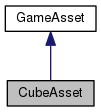
\includegraphics[width=148pt]{classCubeAsset__inherit__graph}
\end{center}
\end{figure}


Collaboration diagram for Cube\+Asset\+:
\nopagebreak
\begin{figure}[H]
\begin{center}
\leavevmode
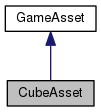
\includegraphics[width=148pt]{classCubeAsset__coll__graph}
\end{center}
\end{figure}
\subsection*{Public Member Functions}
\begin{DoxyCompactItemize}
\item 
\hyperlink{classCubeAsset_ac506cff57e5656238caf95872582d976}{Cube\+Asset} (G\+Lfloat position\+X, G\+Lfloat position\+Y, G\+Lfloat position\+Z)
\item 
\hyperlink{classCubeAsset_ab3ab9a5da82cbf8537a28652410093b1}{$\sim$\+Cube\+Asset} ()
\item 
virtual void \hyperlink{classCubeAsset_a1af568486056e254ffcf98fd99947bfe}{Draw} (G\+Luint)
\end{DoxyCompactItemize}


\subsection{Constructor \& Destructor Documentation}
\hypertarget{classCubeAsset_ac506cff57e5656238caf95872582d976}{}\index{Cube\+Asset@{Cube\+Asset}!Cube\+Asset@{Cube\+Asset}}
\index{Cube\+Asset@{Cube\+Asset}!Cube\+Asset@{Cube\+Asset}}
\subsubsection[{Cube\+Asset(\+G\+Lfloat position\+X, G\+Lfloat position\+Y, G\+Lfloat position\+Z)}]{\setlength{\rightskip}{0pt plus 5cm}Cube\+Asset\+::\+Cube\+Asset (
\begin{DoxyParamCaption}
\item[{G\+Lfloat}]{position\+X, }
\item[{G\+Lfloat}]{position\+Y, }
\item[{G\+Lfloat}]{position\+Z}
\end{DoxyParamCaption}
)}\label{classCubeAsset_ac506cff57e5656238caf95872582d976}
based on the coloured cube tutorial stored float data for the rgb values of the cubes vertices 
\begin{DoxyCode}
5                                                                            \{
6   \textcolor{comment}{// model coordinates, origin at centre.}
7   GLfloat vertex\_buffer\_data [] \{
8         -0.5f + positionX, -0.5f + positionY, -0.5f + positionZ,
9         -0.5f + positionX,  0.5f + positionY, -0.5f + positionZ,
10          0.5f + positionX, -0.5f + positionY, -0.5f + positionZ,
11          0.5f + positionX,  0.5f + positionY, -0.5f + positionZ,
12          0.5f + positionX, -0.5f + positionY,  0.5f + positionZ,
13          0.5f + positionX,  0.5f + positionY,  0.5f + positionZ,
14         -0.5f + positionX, -0.5f + positionY,  0.5f + positionZ,
15         -0.5f + positionX,  0.5f + positionY,  0.5f + positionZ
16   \};
17   GLfloat vertex\_buffer\_length = \textcolor{keyword}{sizeof}(vertex\_buffer\_data);
18 
19 
21    GLfloat g\_colour\_buffer\_data[] = \{
22 
23 
24         0.502f, 0.502f, 0.502f,
25         0.502f, 0.502f, 0.502f,
26         0.502f, 0.502f, 0.502f,
27         0.502f, 0.502f, 0.502f,
28         0.502f, 0.502f, 0.502f,
29         0.502f, 0.502f, 0.502f,
30         0.502f, 0.502f, 0.502f,
31         0.502f, 0.502f, 0.502f
32 
33   \};
34     colour\_buffer\_length = \textcolor{keyword}{sizeof}(g\_colour\_buffer\_data);
35 
36 
37   GLuint element\_buffer []  \{
38         0, 1, 2,
39         1, 3, 2,
40         2, 3, 4,
41         3, 5, 4,
42         0, 2, 4,
43         6, 0, 4,
44         6, 7, 0,
45         1, 0, 7,
46         1, 7, 3,
47         7, 5, 3,
48         5, 6, 4,
49         5, 7, 6
50   \};
51   element\_buffer\_length = \textcolor{keyword}{sizeof}(element\_buffer);
52 
53 
54 
55   \textcolor{comment}{// Transfer buffers to the GPU}
56   \textcolor{comment}{//}
57 
58   \textcolor{comment}{// create buffer}
59   glGenBuffers(1, &vertex\_buffer\_token);
60   \textcolor{comment}{// immediately bind the buffer and transfer the data}
61   glBindBuffer(GL\_ARRAY\_BUFFER, vertex\_buffer\_token);
62   glBufferData(GL\_ARRAY\_BUFFER, vertex\_buffer\_length, vertex\_buffer\_data, GL\_STATIC\_DRAW);
63 
64 
65     glGenBuffers(1, &colour\_buffer\_token);
66     glBindBuffer(GL\_ARRAY\_BUFFER, colour\_buffer\_token);
67     glBufferData(GL\_ARRAY\_BUFFER, colour\_buffer\_length, g\_colour\_buffer\_data, GL\_STATIC\_DRAW);
68 
69 
70   glGenBuffers(1, &element\_buffer\_token);
71   glBindBuffer(GL\_ELEMENT\_ARRAY\_BUFFER, element\_buffer\_token);
72   glBufferData(GL\_ELEMENT\_ARRAY\_BUFFER, element\_buffer\_length, element\_buffer, GL\_STATIC\_DRAW);
73 \}
\end{DoxyCode}
\hypertarget{classCubeAsset_ab3ab9a5da82cbf8537a28652410093b1}{}\index{Cube\+Asset@{Cube\+Asset}!````~Cube\+Asset@{$\sim$\+Cube\+Asset}}
\index{````~Cube\+Asset@{$\sim$\+Cube\+Asset}!Cube\+Asset@{Cube\+Asset}}
\subsubsection[{$\sim$\+Cube\+Asset()}]{\setlength{\rightskip}{0pt plus 5cm}Cube\+Asset\+::$\sim$\+Cube\+Asset (
\begin{DoxyParamCaption}
{}
\end{DoxyParamCaption}
)}\label{classCubeAsset_ab3ab9a5da82cbf8537a28652410093b1}

\begin{DoxyCode}
75                       \{
76 \}
\end{DoxyCode}


\subsection{Member Function Documentation}
\hypertarget{classCubeAsset_a1af568486056e254ffcf98fd99947bfe}{}\index{Cube\+Asset@{Cube\+Asset}!Draw@{Draw}}
\index{Draw@{Draw}!Cube\+Asset@{Cube\+Asset}}
\subsubsection[{Draw(\+G\+Luint)}]{\setlength{\rightskip}{0pt plus 5cm}void Cube\+Asset\+::\+Draw (
\begin{DoxyParamCaption}
\item[{G\+Luint}]{program\+\_\+token}
\end{DoxyParamCaption}
)\hspace{0.3cm}{\ttfamily [virtual]}}\label{classCubeAsset_a1af568486056e254ffcf98fd99947bfe}


Implements \hyperlink{classGameAsset_a961aa51ca0a9961fc584c0b5d5431300}{Game\+Asset}.


\begin{DoxyCode}
93                                          \{
94   \textcolor{keywordflow}{if}(!glIsProgram(program\_token)) \{
95     std::cerr << \textcolor{stringliteral}{"Drawing Cube with invalid program"} << std::endl;
96     \textcolor{keywordflow}{return};
97   \}
98   GLint validation\_ok;
99   glValidateProgram(program\_token);
100   glGetProgramiv(program\_token, GL\_VALIDATE\_STATUS, &validation\_ok);
101   \textcolor{keywordflow}{if}(!validation\_ok) \{
102     GLint maxLength = 0;
103     glGetProgramiv(program\_token, GL\_INFO\_LOG\_LENGTH, &maxLength);
104 
105     \textcolor{comment}{//The maxLength includes the NULL character}
106     std::vector<char> errorLog(maxLength);
107     glGetProgramInfoLog(program\_token, maxLength, &maxLength, &errorLog[0]);
108 
109     std::cerr << \textcolor{stringliteral}{"Invalid program "} << program\_token << \textcolor{stringliteral}{" with error code "} << validation\_ok << std::endl;
110     \textcolor{keywordflow}{for}(\textcolor{keyword}{auto} c: errorLog) \{
111       std::cerr << c;
112     \}
113     exit(-1);
114   \}
115 
116   GLuint position\_attrib = glGetAttribLocation(program\_token, \textcolor{stringliteral}{"position"});
117   \hyperlink{CubeAsset_8cc_a75f201b0e53e68726854997957322b8d}{checkGLError}();
118 
119   glUseProgram(program\_token);
120   \hyperlink{CubeAsset_8cc_a75f201b0e53e68726854997957322b8d}{checkGLError}();
121 
122   \textcolor{comment}{// use the previously transferred buffer as the vertex array.  This way}
123   \textcolor{comment}{// we transfer the buffer once -- at construction -- not on every frame.}
124   glEnableVertexAttribArray(0);
125   glBindBuffer(GL\_ARRAY\_BUFFER, vertex\_buffer\_token);
126   glVertexAttribPointer(
127     0,        \textcolor{comment}{/* attribute */}
128     3,        \textcolor{comment}{/* size */}
129     GL\_FLOAT,   \textcolor{comment}{/* type */}
130     GL\_FALSE,   \textcolor{comment}{/* normalized? */}
131     0,        \textcolor{comment}{/* stride */}
132     (\textcolor{keywordtype}{void}*)0    \textcolor{comment}{/* array buffer offset */}
133   );
134   glEnableVertexAttribArray(1);
135   \hyperlink{CubeAsset_8cc_a75f201b0e53e68726854997957322b8d}{checkGLError}();
136 
137   glBindBuffer(GL\_ARRAY\_BUFFER, colour\_buffer\_token);
138   glVertexAttribPointer(
139     1,        \textcolor{comment}{/* attribute */}
140     3,        \textcolor{comment}{/* size */}
141     GL\_FLOAT,   \textcolor{comment}{/* type */}
142     GL\_FALSE,   \textcolor{comment}{/* normalized? */}
143     0,        \textcolor{comment}{/* stride */}
144     (\textcolor{keywordtype}{void}*)0    \textcolor{comment}{/* array buffer offset */}
145   );
146   \hyperlink{CubeAsset_8cc_a75f201b0e53e68726854997957322b8d}{checkGLError}();
147 
148   glBindBuffer(GL\_ELEMENT\_ARRAY\_BUFFER, element\_buffer\_token);
149   glDrawElements(
150     GL\_TRIANGLES,
151     element\_buffer\_length,
152     GL\_UNSIGNED\_INT,
153     (GLvoid*) 0
154   );
155   \hyperlink{CubeAsset_8cc_a75f201b0e53e68726854997957322b8d}{checkGLError}();
156 
157   glDisableVertexAttribArray(position\_attrib);
158 \}
\end{DoxyCode}


The documentation for this class was generated from the following files\+:\begin{DoxyCompactItemize}
\item 
src/\hyperlink{CubeAsset_8h}{Cube\+Asset.\+h}\item 
src/\hyperlink{CubeAsset_8cc}{Cube\+Asset.\+cc}\end{DoxyCompactItemize}

\hypertarget{classDiamondAsset}{}\section{Diamond\+Asset Class Reference}
\label{classDiamondAsset}\index{Diamond\+Asset@{Diamond\+Asset}}
Inheritance diagram for Diamond\+Asset\+:\begin{figure}[H]
\begin{center}
\leavevmode
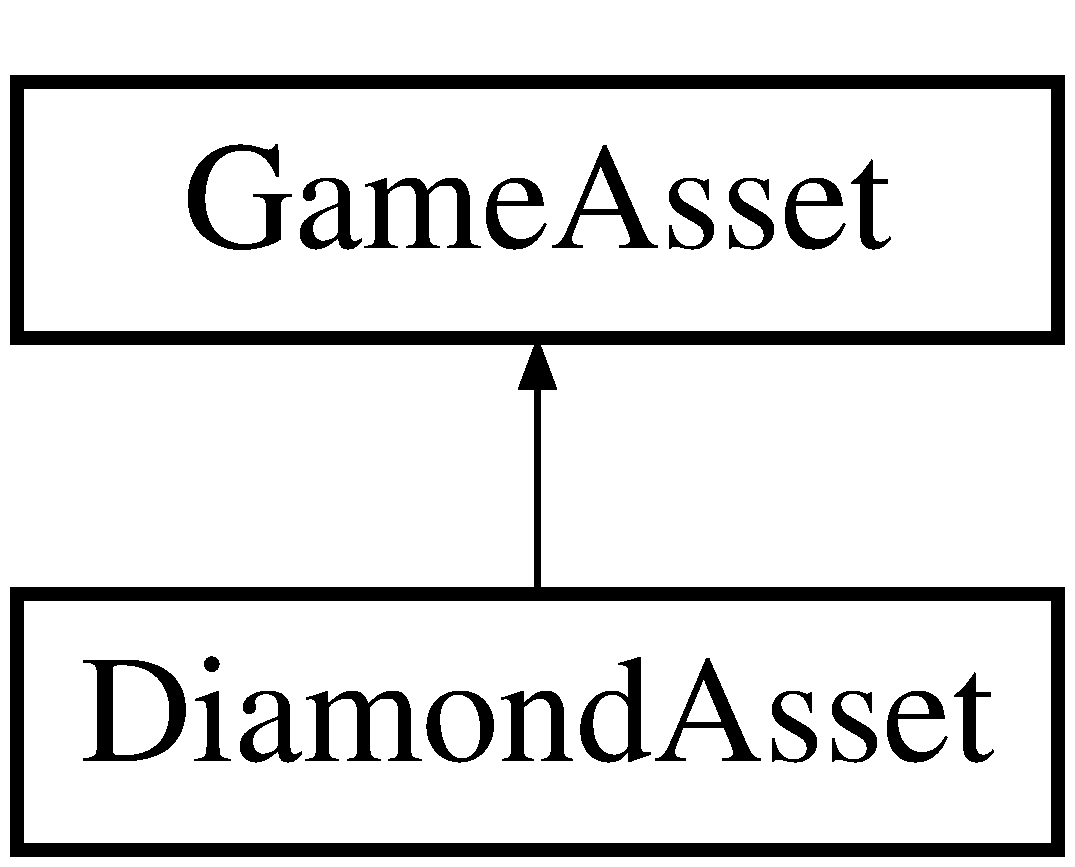
\includegraphics[height=2.000000cm]{classDiamondAsset}
\end{center}
\end{figure}
\subsection*{Public Member Functions}
\begin{DoxyCompactItemize}
\item 
\hyperlink{classDiamondAsset_a8023636a5affbf3f7347908a1891d02e}{Diamond\+Asset} (glm\+::vec3, glm\+::vec3, int, float, glm\+::vec3, glm\+::vec3)
\item 
\hyperlink{classDiamondAsset_a1b7bf6ba76651a9304943f2c41fe36b8}{$\sim$\+Diamond\+Asset} ()
\end{DoxyCompactItemize}
\subsection*{Additional Inherited Members}


\subsection{Constructor \& Destructor Documentation}
\hypertarget{classDiamondAsset_a8023636a5affbf3f7347908a1891d02e}{}\index{Diamond\+Asset@{Diamond\+Asset}!Diamond\+Asset@{Diamond\+Asset}}
\index{Diamond\+Asset@{Diamond\+Asset}!Diamond\+Asset@{Diamond\+Asset}}
\subsubsection[{Diamond\+Asset(glm\+::vec3, glm\+::vec3, int, float, glm\+::vec3, glm\+::vec3)}]{\setlength{\rightskip}{0pt plus 5cm}Diamond\+Asset\+::\+Diamond\+Asset (
\begin{DoxyParamCaption}
\item[{glm\+::vec3}]{p, }
\item[{glm\+::vec3}]{c, }
\item[{int}]{type, }
\item[{float}]{scale, }
\item[{glm\+::vec3}]{rotation, }
\item[{glm\+::vec3}]{speed}
\end{DoxyParamCaption}
)}\label{classDiamondAsset_a8023636a5affbf3f7347908a1891d02e}
Heavily modified from the original. Initialisation for the asset 
\begin{DoxyParams}{Parameters}
{\em glm\+::vec3} & p\+: The asset initial position \\
\hline
{\em glm\+::vec3} & c\+: The asset colour \\
\hline
{\em int} & type\+: What action to perform, check Bounding\+Box.\+cc for the types \\
\hline
{\em float} & scale\+: Initialisation scale/size of the asset. (1 will create it at normal size, lower = smaller, higher = larger) \\
\hline
{\em glm\+::vec3} & rotation\+: Initialises the asset rotated if the vec3 is more than (0.\+0f,0.\+0f,0.\+0f) \\
\hline
{\em glm\+::vev3} & speed\+: Initialises the asset translating towards a point. \\
\hline
\end{DoxyParams}
Transfer buffers to the G\+P\+U create buffer immediately bind the buffer and transfer the data\hypertarget{classDiamondAsset_a1b7bf6ba76651a9304943f2c41fe36b8}{}\index{Diamond\+Asset@{Diamond\+Asset}!````~Diamond\+Asset@{$\sim$\+Diamond\+Asset}}
\index{````~Diamond\+Asset@{$\sim$\+Diamond\+Asset}!Diamond\+Asset@{Diamond\+Asset}}
\subsubsection[{$\sim$\+Diamond\+Asset()}]{\setlength{\rightskip}{0pt plus 5cm}Diamond\+Asset\+::$\sim$\+Diamond\+Asset (
\begin{DoxyParamCaption}
{}
\end{DoxyParamCaption}
)}\label{classDiamondAsset_a1b7bf6ba76651a9304943f2c41fe36b8}
Class destructor method 

The documentation for this class was generated from the following files\+:\begin{DoxyCompactItemize}
\item 
Diamond\+Asset.\+h\item 
Diamond\+Asset.\+cc\end{DoxyCompactItemize}

\hypertarget{classGameAsset}{}\section{Game\+Asset Class Reference}
\label{classGameAsset}\index{Game\+Asset@{Game\+Asset}}


{\ttfamily \#include $<$Game\+Asset.\+h$>$}



Inheritance diagram for Game\+Asset\+:
\nopagebreak
\begin{figure}[H]
\begin{center}
\leavevmode
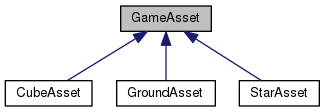
\includegraphics[width=316pt]{classGameAsset__inherit__graph}
\end{center}
\end{figure}
\subsection*{Public Member Functions}
\begin{DoxyCompactItemize}
\item 
virtual void \hyperlink{classGameAsset_a961aa51ca0a9961fc584c0b5d5431300}{Draw} (G\+Luint)=0
\end{DoxyCompactItemize}


\subsection{Member Function Documentation}
\hypertarget{classGameAsset_a961aa51ca0a9961fc584c0b5d5431300}{}\index{Game\+Asset@{Game\+Asset}!Draw@{Draw}}
\index{Draw@{Draw}!Game\+Asset@{Game\+Asset}}
\subsubsection[{Draw(\+G\+Luint)=0}]{\setlength{\rightskip}{0pt plus 5cm}virtual void Game\+Asset\+::\+Draw (
\begin{DoxyParamCaption}
\item[{G\+Luint}]{}
\end{DoxyParamCaption}
)\hspace{0.3cm}{\ttfamily [pure virtual]}}\label{classGameAsset_a961aa51ca0a9961fc584c0b5d5431300}


Implemented in \hyperlink{classCubeAsset_a1af568486056e254ffcf98fd99947bfe}{Cube\+Asset}, \hyperlink{classGroundAsset_a440f983638c7a7ccb6a39718444dfe95}{Ground\+Asset}, and \hyperlink{classStarAsset_a1e44c9446a0443f8f7fdddf9fb74b8d7}{Star\+Asset}.



The documentation for this class was generated from the following file\+:\begin{DoxyCompactItemize}
\item 
src/\hyperlink{GameAsset_8h}{Game\+Asset.\+h}\end{DoxyCompactItemize}

\hypertarget{classGameAssetManager}{}\section{Game\+Asset\+Manager Class Reference}
\label{classGameAssetManager}\index{Game\+Asset\+Manager@{Game\+Asset\+Manager}}


{\ttfamily \#include $<$Game\+Asset\+Manager.\+h$>$}

\subsection*{Public Member Functions}
\begin{DoxyCompactItemize}
\item 
\hyperlink{classGameAssetManager_a84d0445928649e0d1e0f8e31ee137b17}{Game\+Asset\+Manager} ()
\item 
virtual \hyperlink{classGameAssetManager_a1270bd61ecbcca563f079803e40c9b77}{$\sim$\+Game\+Asset\+Manager} ()
\item 
\hyperlink{classGameAssetManager_a2c9adcb72faa154c87eadc9bafe5269d}{Game\+Asset\+Manager} (\hyperlink{classGameAssetManager}{Game\+Asset\+Manager} const \&)
\item 
\hyperlink{classGameAssetManager_a44f6e2fd6b8ff1dd64e5697f1be7386d}{Game\+Asset\+Manager} (\hyperlink{classGameAssetManager}{Game\+Asset\+Manager} const \&\&)
\item 
void \hyperlink{classGameAssetManager_ac72678a4ad5378c685aa6bae84a4e712}{operator=} (\hyperlink{classGameAssetManager}{Game\+Asset\+Manager} const \&)
\item 
void \hyperlink{classGameAssetManager_ad3de8ff00d55ba04728b1de8213b2349}{Add\+Asset} (std\+::shared\+\_\+ptr$<$ \hyperlink{classGameAsset}{Game\+Asset} $>$)
\item 
void \hyperlink{classGameAssetManager_a0627c08b5696fac9ebf3076b5766599b}{Delete\+Asset} (glm\+::vec3)
\item 
void \hyperlink{classGameAssetManager_a7898abe62096f7de7d04e1e4c22f0f87}{Set\+Path} (glm\+::vec3, bool)
\item 
void \hyperlink{classGameAssetManager_a32837132bd70a9a9ed537323c2d3d886}{Draw} ()
\item 
void \hyperlink{classGameAssetManager_aeb9a8c013f49f2ab06a51b5033576061}{Update\+Camera\+Position} (Input, int, int)
\item 
glm\+::vec3 \hyperlink{classGameAssetManager_a1d9f1f5cc6630a10a0bf358dc2bcddef}{Get\+Camera\+Position} ()
\item 
glm\+::vec3 \hyperlink{classGameAssetManager_a236ee25b1346115f0ee68f1497b02e85}{Get\+Camera\+Direction} ()
\end{DoxyCompactItemize}
\subsection*{Public Attributes}
\begin{DoxyCompactItemize}
\item 
\hypertarget{classGameAssetManager_a01330dececa65c4a5da1be683c14969c}{}std\+::vector$<$ glm\+::vec3 $>$ {\bfseries path\+\_\+list}\label{classGameAssetManager_a01330dececa65c4a5da1be683c14969c}

\end{DoxyCompactItemize}


\subsection{Detailed Description}
\hyperlink{classGameAssetManager}{Game\+Asset\+Manager} is a container for Game\+Assets. It also provides utility functions to to create a simple Open\+G\+L program that can be used to draw a simple \hyperlink{classGameAsset}{Game\+Asset}. 

\subsection{Constructor \& Destructor Documentation}
\hypertarget{classGameAssetManager_a84d0445928649e0d1e0f8e31ee137b17}{}\index{Game\+Asset\+Manager@{Game\+Asset\+Manager}!Game\+Asset\+Manager@{Game\+Asset\+Manager}}
\index{Game\+Asset\+Manager@{Game\+Asset\+Manager}!Game\+Asset\+Manager@{Game\+Asset\+Manager}}
\subsubsection[{Game\+Asset\+Manager()}]{\setlength{\rightskip}{0pt plus 5cm}Game\+Asset\+Manager\+::\+Game\+Asset\+Manager (
\begin{DoxyParamCaption}
{}
\end{DoxyParamCaption}
)}\label{classGameAssetManager_a84d0445928649e0d1e0f8e31ee137b17}
Creates a \hyperlink{classGameAssetManager}{Game\+Asset\+Manager} to load the correct shaders based on the Application\+Mode. \hypertarget{classGameAssetManager_a1270bd61ecbcca563f079803e40c9b77}{}\index{Game\+Asset\+Manager@{Game\+Asset\+Manager}!````~Game\+Asset\+Manager@{$\sim$\+Game\+Asset\+Manager}}
\index{````~Game\+Asset\+Manager@{$\sim$\+Game\+Asset\+Manager}!Game\+Asset\+Manager@{Game\+Asset\+Manager}}
\subsubsection[{$\sim$\+Game\+Asset\+Manager()}]{\setlength{\rightskip}{0pt plus 5cm}Game\+Asset\+Manager\+::$\sim$\+Game\+Asset\+Manager (
\begin{DoxyParamCaption}
{}
\end{DoxyParamCaption}
)\hspace{0.3cm}{\ttfamily [virtual]}}\label{classGameAssetManager_a1270bd61ecbcca563f079803e40c9b77}
Deletes a \hyperlink{classGameAssetManager}{Game\+Asset\+Manager}, in particular it will clean up any modifications to the Open\+G\+L state. \hypertarget{classGameAssetManager_a2c9adcb72faa154c87eadc9bafe5269d}{}\index{Game\+Asset\+Manager@{Game\+Asset\+Manager}!Game\+Asset\+Manager@{Game\+Asset\+Manager}}
\index{Game\+Asset\+Manager@{Game\+Asset\+Manager}!Game\+Asset\+Manager@{Game\+Asset\+Manager}}
\subsubsection[{Game\+Asset\+Manager(\+Game\+Asset\+Manager const \&)}]{\setlength{\rightskip}{0pt plus 5cm}Game\+Asset\+Manager\+::\+Game\+Asset\+Manager (
\begin{DoxyParamCaption}
\item[{{\bf Game\+Asset\+Manager} const \&}]{the\+\_\+manager}
\end{DoxyParamCaption}
)}\label{classGameAssetManager_a2c9adcb72faa154c87eadc9bafe5269d}
Unimplemented copy constructor -- this means that the \hyperlink{classGameAssetManager}{Game\+Asset\+Manager} may not work as you\textquotesingle{}d expect when being copied. \hypertarget{classGameAssetManager_a44f6e2fd6b8ff1dd64e5697f1be7386d}{}\index{Game\+Asset\+Manager@{Game\+Asset\+Manager}!Game\+Asset\+Manager@{Game\+Asset\+Manager}}
\index{Game\+Asset\+Manager@{Game\+Asset\+Manager}!Game\+Asset\+Manager@{Game\+Asset\+Manager}}
\subsubsection[{Game\+Asset\+Manager(\+Game\+Asset\+Manager const \&\&)}]{\setlength{\rightskip}{0pt plus 5cm}Game\+Asset\+Manager\+::\+Game\+Asset\+Manager (
\begin{DoxyParamCaption}
\item[{{\bf Game\+Asset\+Manager} const \&\&}]{the\+\_\+manager}
\end{DoxyParamCaption}
)}\label{classGameAssetManager_a44f6e2fd6b8ff1dd64e5697f1be7386d}
Unimplemented move constructor -- this unimplemented method violates the C++11 move semantics for \hyperlink{classGameAssetManager}{Game\+Asset\+Manager}. 

\subsection{Member Function Documentation}
\hypertarget{classGameAssetManager_ad3de8ff00d55ba04728b1de8213b2349}{}\index{Game\+Asset\+Manager@{Game\+Asset\+Manager}!Add\+Asset@{Add\+Asset}}
\index{Add\+Asset@{Add\+Asset}!Game\+Asset\+Manager@{Game\+Asset\+Manager}}
\subsubsection[{Add\+Asset(std\+::shared\+\_\+ptr$<$ Game\+Asset $>$)}]{\setlength{\rightskip}{0pt plus 5cm}void Game\+Asset\+Manager\+::\+Add\+Asset (
\begin{DoxyParamCaption}
\item[{std\+::shared\+\_\+ptr$<$ {\bf Game\+Asset} $>$}]{the\+\_\+asset}
\end{DoxyParamCaption}
)}\label{classGameAssetManager_ad3de8ff00d55ba04728b1de8213b2349}
Adds a \hyperlink{classGameAsset}{Game\+Asset} to the scene graph. \hypertarget{classGameAssetManager_a0627c08b5696fac9ebf3076b5766599b}{}\index{Game\+Asset\+Manager@{Game\+Asset\+Manager}!Delete\+Asset@{Delete\+Asset}}
\index{Delete\+Asset@{Delete\+Asset}!Game\+Asset\+Manager@{Game\+Asset\+Manager}}
\subsubsection[{Delete\+Asset(glm\+::vec3)}]{\setlength{\rightskip}{0pt plus 5cm}void Game\+Asset\+Manager\+::\+Delete\+Asset (
\begin{DoxyParamCaption}
\item[{glm\+::vec3}]{position}
\end{DoxyParamCaption}
)}\label{classGameAssetManager_a0627c08b5696fac9ebf3076b5766599b}
Deletes an asset from the draw\+\_\+list \hypertarget{classGameAssetManager_a32837132bd70a9a9ed537323c2d3d886}{}\index{Game\+Asset\+Manager@{Game\+Asset\+Manager}!Draw@{Draw}}
\index{Draw@{Draw}!Game\+Asset\+Manager@{Game\+Asset\+Manager}}
\subsubsection[{Draw()}]{\setlength{\rightskip}{0pt plus 5cm}void Game\+Asset\+Manager\+::\+Draw (
\begin{DoxyParamCaption}
{}
\end{DoxyParamCaption}
)}\label{classGameAssetManager_a32837132bd70a9a9ed537323c2d3d886}
Draws each \hyperlink{classGameAsset}{Game\+Asset} in the scene graph. \hypertarget{classGameAssetManager_a236ee25b1346115f0ee68f1497b02e85}{}\index{Game\+Asset\+Manager@{Game\+Asset\+Manager}!Get\+Camera\+Direction@{Get\+Camera\+Direction}}
\index{Get\+Camera\+Direction@{Get\+Camera\+Direction}!Game\+Asset\+Manager@{Game\+Asset\+Manager}}
\subsubsection[{Get\+Camera\+Direction()}]{\setlength{\rightskip}{0pt plus 5cm}glm\+::vec3 Game\+Asset\+Manager\+::\+Get\+Camera\+Direction (
\begin{DoxyParamCaption}
{}
\end{DoxyParamCaption}
)}\label{classGameAssetManager_a236ee25b1346115f0ee68f1497b02e85}
Fetches and returns the camera direction \hypertarget{classGameAssetManager_a1d9f1f5cc6630a10a0bf358dc2bcddef}{}\index{Game\+Asset\+Manager@{Game\+Asset\+Manager}!Get\+Camera\+Position@{Get\+Camera\+Position}}
\index{Get\+Camera\+Position@{Get\+Camera\+Position}!Game\+Asset\+Manager@{Game\+Asset\+Manager}}
\subsubsection[{Get\+Camera\+Position()}]{\setlength{\rightskip}{0pt plus 5cm}glm\+::vec3 Game\+Asset\+Manager\+::\+Get\+Camera\+Position (
\begin{DoxyParamCaption}
{}
\end{DoxyParamCaption}
)}\label{classGameAssetManager_a1d9f1f5cc6630a10a0bf358dc2bcddef}
Fetches and returns the camera position \hypertarget{classGameAssetManager_ac72678a4ad5378c685aa6bae84a4e712}{}\index{Game\+Asset\+Manager@{Game\+Asset\+Manager}!operator=@{operator=}}
\index{operator=@{operator=}!Game\+Asset\+Manager@{Game\+Asset\+Manager}}
\subsubsection[{operator=(\+Game\+Asset\+Manager const \&)}]{\setlength{\rightskip}{0pt plus 5cm}void Game\+Asset\+Manager\+::operator= (
\begin{DoxyParamCaption}
\item[{{\bf Game\+Asset\+Manager} const \&}]{the\+\_\+manager}
\end{DoxyParamCaption}
)}\label{classGameAssetManager_ac72678a4ad5378c685aa6bae84a4e712}
Unimplemented assisgnment operator -- violates the expected semantics for assignment in C++11. \hypertarget{classGameAssetManager_a7898abe62096f7de7d04e1e4c22f0f87}{}\index{Game\+Asset\+Manager@{Game\+Asset\+Manager}!Set\+Path@{Set\+Path}}
\index{Set\+Path@{Set\+Path}!Game\+Asset\+Manager@{Game\+Asset\+Manager}}
\subsubsection[{Set\+Path(glm\+::vec3, bool)}]{\setlength{\rightskip}{0pt plus 5cm}void Game\+Asset\+Manager\+::\+Set\+Path (
\begin{DoxyParamCaption}
\item[{glm\+::vec3}]{path, }
\item[{bool}]{active}
\end{DoxyParamCaption}
)}\label{classGameAssetManager_a7898abe62096f7de7d04e1e4c22f0f87}
Gives a game\+Asset some path Coordinates \hypertarget{classGameAssetManager_aeb9a8c013f49f2ab06a51b5033576061}{}\index{Game\+Asset\+Manager@{Game\+Asset\+Manager}!Update\+Camera\+Position@{Update\+Camera\+Position}}
\index{Update\+Camera\+Position@{Update\+Camera\+Position}!Game\+Asset\+Manager@{Game\+Asset\+Manager}}
\subsubsection[{Update\+Camera\+Position(\+Input, int, int)}]{\setlength{\rightskip}{0pt plus 5cm}void Game\+Asset\+Manager\+::\+Update\+Camera\+Position (
\begin{DoxyParamCaption}
\item[{Input}]{input\+\_\+direction, }
\item[{int}]{mouse\+\_\+x, }
\item[{int}]{mouse\+\_\+y}
\end{DoxyParamCaption}
)}\label{classGameAssetManager_aeb9a8c013f49f2ab06a51b5033576061}
Communicates with \hyperlink{classCamera}{Camera} class 

The documentation for this class was generated from the following files\+:\begin{DoxyCompactItemize}
\item 
Game\+Asset\+Manager.\+h\item 
Game\+Asset\+Manager.\+cc\end{DoxyCompactItemize}

\hypertarget{classGameWorld}{}\section{Game\+World Class Reference}
\label{classGameWorld}\index{Game\+World@{Game\+World}}


{\ttfamily \#include $<$Game\+World.\+h$>$}

\subsection*{Public Member Functions}
\begin{DoxyCompactItemize}
\item 
\hyperlink{classGameWorld_a681994123c12833d43c957d6cfb33765}{Game\+World} ()
\item 
void \hyperlink{classGameWorld_a275418607d8286979b276f165ad5876b}{Draw} ()
\item 
void \hyperlink{classGameWorld_a9b394b1c980a7735476eb80171642108}{Update\+Camera\+Position} (Input, int, int)
\item 
void \hyperlink{classGameWorld_ac4ad43a43be6e6eb7ee311173783873c}{Block\+Action} (bool)
\item 
void \hyperlink{classGameWorld_a92aa1f5e8a65a688f1d030f22d867ccc}{Block\+Type} (Asset\+Type)
\end{DoxyCompactItemize}


\subsection{Detailed Description}
\hyperlink{classGameWorld}{Game\+World} allows us to separate the management of the game world from the nuts and bolts of game loop initialisation. The \hyperlink{classGameWorld}{Game\+World} currently has a very simplified scene graph consisiting of a single \hyperlink{classGameAssetManager}{Game\+Asset\+Manager}. 

\subsection{Constructor \& Destructor Documentation}
\hypertarget{classGameWorld_a681994123c12833d43c957d6cfb33765}{}\index{Game\+World@{Game\+World}!Game\+World@{Game\+World}}
\index{Game\+World@{Game\+World}!Game\+World@{Game\+World}}
\subsubsection[{Game\+World()}]{\setlength{\rightskip}{0pt plus 5cm}Game\+World\+::\+Game\+World (
\begin{DoxyParamCaption}
{}
\end{DoxyParamCaption}
)}\label{classGameWorld_a681994123c12833d43c957d6cfb33765}
We thread the Application\+Mode through the \hyperlink{classGameWorld}{Game\+World} ss we want to read it in from the user. Threading the state through the various function calls is preferable (in this case) to having some kind of global state.

Initialises the \hyperlink{classGameWorld}{Game\+World} Places some blocks within the \hyperlink{classGameWorld}{Game\+World} to demonstrate all of the available animation and key-\/frame features Assets that are sitting on the spot, but performing an action (Such as Translate, Rotate and Scale)

Assets that are using \char`\"{}path\char`\"{}/\char`\"{}key-\/frames\char`\"{}

\subsection{Member Function Documentation}
\hypertarget{classGameWorld_ac4ad43a43be6e6eb7ee311173783873c}{}\index{Game\+World@{Game\+World}!Block\+Action@{Block\+Action}}
\index{Block\+Action@{Block\+Action}!Game\+World@{Game\+World}}
\subsubsection[{Block\+Action(bool)}]{\setlength{\rightskip}{0pt plus 5cm}void Game\+World\+::\+Block\+Action (
\begin{DoxyParamCaption}
\item[{bool}]{mode}
\end{DoxyParamCaption}
)}\label{classGameWorld_ac4ad43a43be6e6eb7ee311173783873c}
Add and remove cubes from the game world \hypertarget{classGameWorld_a92aa1f5e8a65a688f1d030f22d867ccc}{}\index{Game\+World@{Game\+World}!Block\+Type@{Block\+Type}}
\index{Block\+Type@{Block\+Type}!Game\+World@{Game\+World}}
\subsubsection[{Block\+Type(\+Asset\+Type)}]{\setlength{\rightskip}{0pt plus 5cm}void Game\+World\+::\+Block\+Type (
\begin{DoxyParamCaption}
\item[{Asset\+Type}]{type}
\end{DoxyParamCaption}
)}\label{classGameWorld_a92aa1f5e8a65a688f1d030f22d867ccc}
Changes the type of asset to make based on user input \hypertarget{classGameWorld_a275418607d8286979b276f165ad5876b}{}\index{Game\+World@{Game\+World}!Draw@{Draw}}
\index{Draw@{Draw}!Game\+World@{Game\+World}}
\subsubsection[{Draw()}]{\setlength{\rightskip}{0pt plus 5cm}void Game\+World\+::\+Draw (
\begin{DoxyParamCaption}
{}
\end{DoxyParamCaption}
)}\label{classGameWorld_a275418607d8286979b276f165ad5876b}
Calling \hyperlink{classGameWorld_a275418607d8286979b276f165ad5876b}{Draw()} will draw the entire world.

Calls \hyperlink{classGameAssetManager}{Game\+Asset\+Manager} Drawing method \hypertarget{classGameWorld_a9b394b1c980a7735476eb80171642108}{}\index{Game\+World@{Game\+World}!Update\+Camera\+Position@{Update\+Camera\+Position}}
\index{Update\+Camera\+Position@{Update\+Camera\+Position}!Game\+World@{Game\+World}}
\subsubsection[{Update\+Camera\+Position(\+Input, int, int)}]{\setlength{\rightskip}{0pt plus 5cm}void Game\+World\+::\+Update\+Camera\+Position (
\begin{DoxyParamCaption}
\item[{Input}]{input\+\_\+direction, }
\item[{int}]{mouse\+\_\+x, }
\item[{int}]{mouse\+\_\+y}
\end{DoxyParamCaption}
)}\label{classGameWorld_a9b394b1c980a7735476eb80171642108}
Calls the Update\+Camera\+Position method in \hyperlink{classGameAssetManager}{Game\+Asset\+Manager} passing the user input and mouse coordnates. 

The documentation for this class was generated from the following files\+:\begin{DoxyCompactItemize}
\item 
Game\+World.\+h\item 
Game\+World.\+cc\end{DoxyCompactItemize}

\hypertarget{classPythonBindings}{}\section{Python\+Bindings Class Reference}
\label{classPythonBindings}\index{Python\+Bindings@{Python\+Bindings}}
\subsection*{Public Member Functions}
\begin{DoxyCompactItemize}
\item 
\hyperlink{classPythonBindings_acd1e5f8c23f2817736d9d4a07e4988a9}{Python\+Bindings} ()
\end{DoxyCompactItemize}


\subsection{Constructor \& Destructor Documentation}
\hypertarget{classPythonBindings_acd1e5f8c23f2817736d9d4a07e4988a9}{}\index{Python\+Bindings@{Python\+Bindings}!Python\+Bindings@{Python\+Bindings}}
\index{Python\+Bindings@{Python\+Bindings}!Python\+Bindings@{Python\+Bindings}}
\subsubsection[{Python\+Bindings()}]{\setlength{\rightskip}{0pt plus 5cm}Python\+Bindings\+::\+Python\+Bindings (
\begin{DoxyParamCaption}
{}
\end{DoxyParamCaption}
)}\label{classPythonBindings_acd1e5f8c23f2817736d9d4a07e4988a9}
Class constructor 

The documentation for this class was generated from the following files\+:\begin{DoxyCompactItemize}
\item 
Python\+Bindings.\+h\item 
Python\+Bindings.\+cc\end{DoxyCompactItemize}

\hypertarget{structSDLWindowDeleter}{}\section{S\+D\+L\+Window\+Deleter Struct Reference}
\label{structSDLWindowDeleter}\index{S\+D\+L\+Window\+Deleter@{S\+D\+L\+Window\+Deleter}}
\subsection*{Public Member Functions}
\begin{DoxyCompactItemize}
\item 
void \hyperlink{structSDLWindowDeleter_a2aedcc99c3756ae090c38badabeb10b1}{operator()} (S\+D\+L\+\_\+\+Window $\ast$window)
\end{DoxyCompactItemize}


\subsection{Member Function Documentation}
\hypertarget{structSDLWindowDeleter_a2aedcc99c3756ae090c38badabeb10b1}{}\index{S\+D\+L\+Window\+Deleter@{S\+D\+L\+Window\+Deleter}!operator()@{operator()}}
\index{operator()@{operator()}!S\+D\+L\+Window\+Deleter@{S\+D\+L\+Window\+Deleter}}
\subsubsection[{operator()(\+S\+D\+L\+\_\+\+Window $\ast$window)}]{\setlength{\rightskip}{0pt plus 5cm}void S\+D\+L\+Window\+Deleter\+::operator() (
\begin{DoxyParamCaption}
\item[{S\+D\+L\+\_\+\+Window $\ast$}]{window}
\end{DoxyParamCaption}
)\hspace{0.3cm}{\ttfamily [inline]}}\label{structSDLWindowDeleter_a2aedcc99c3756ae090c38badabeb10b1}

\begin{DoxyCode}
32                                              \{
33     SDL\_DestroyWindow(window);
34   \}
\end{DoxyCode}


The documentation for this struct was generated from the following file\+:\begin{DoxyCompactItemize}
\item 
src/\hyperlink{main_8cc}{main.\+cc}\end{DoxyCompactItemize}

\hypertarget{classStarAsset}{}\section{Star\+Asset Class Reference}
\label{classStarAsset}\index{Star\+Asset@{Star\+Asset}}


{\ttfamily \#include $<$Star\+Asset.\+h$>$}



Inheritance diagram for Star\+Asset\+:
\nopagebreak
\begin{figure}[H]
\begin{center}
\leavevmode
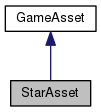
\includegraphics[width=148pt]{classStarAsset__inherit__graph}
\end{center}
\end{figure}


Collaboration diagram for Star\+Asset\+:
\nopagebreak
\begin{figure}[H]
\begin{center}
\leavevmode
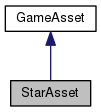
\includegraphics[width=148pt]{classStarAsset__coll__graph}
\end{center}
\end{figure}
\subsection*{Public Member Functions}
\begin{DoxyCompactItemize}
\item 
\hyperlink{classStarAsset_aa97b2aacfe7fba0f042076a045b96c43}{Star\+Asset} (G\+Lfloat position\+X, G\+Lfloat position\+Y, G\+Lfloat position\+Z)
\item 
\hyperlink{classStarAsset_a77a07269f87ab84c206d1bc5733e0a10}{$\sim$\+Star\+Asset} ()
\item 
virtual void \hyperlink{classStarAsset_a1e44c9446a0443f8f7fdddf9fb74b8d7}{Draw} (G\+Luint)
\end{DoxyCompactItemize}


\subsection{Constructor \& Destructor Documentation}
\hypertarget{classStarAsset_aa97b2aacfe7fba0f042076a045b96c43}{}\index{Star\+Asset@{Star\+Asset}!Star\+Asset@{Star\+Asset}}
\index{Star\+Asset@{Star\+Asset}!Star\+Asset@{Star\+Asset}}
\subsubsection[{Star\+Asset(\+G\+Lfloat position\+X, G\+Lfloat position\+Y, G\+Lfloat position\+Z)}]{\setlength{\rightskip}{0pt plus 5cm}Star\+Asset\+::\+Star\+Asset (
\begin{DoxyParamCaption}
\item[{G\+Lfloat}]{position\+X, }
\item[{G\+Lfloat}]{position\+Y, }
\item[{G\+Lfloat}]{position\+Z}
\end{DoxyParamCaption}
)}\label{classStarAsset_aa97b2aacfe7fba0f042076a045b96c43}

\begin{DoxyCode}
5                                                                            \{
6   \textcolor{comment}{// model coordinates, origin at centre.}
7   GLfloat vertex\_buffer\_data [] \{
8         
9                 0.0f  + positionX, 1.0f     + positionY, 0.5f + positionZ,
10         -0.25f + positionX, 0.25f  + positionY, 0.5f + positionZ,
11         0.25f  + positionX, 0.25f  + positionY, 0.5f + positionZ,
12         -1.0f    + positionX, 0.0f   + positionY, 0.5f + positionZ,
13         0.0f   + positionX, 0.0f   + positionY, 0.5f + positionZ,
14         1.0f     + positionX, 0.0f   + positionY, 0.5f + positionZ,
15         -0.25f + positionX, -0.25f + positionY, 0.5f + positionZ,
16         0.25f  + positionX, -0.25f + positionY, 0.5f + positionZ,
17         0.0f   + positionX, -1.0f    + positionY, 0.5f + positionZ
18   \};
19   GLfloat vertex\_buffer\_length = \textcolor{keyword}{sizeof}(vertex\_buffer\_data);
20 
21    GLfloat g\_colour\_buffer\_data[] = \{
22 1.000f, 1.000f, 0.000f,
23 1.000f, 1.000f, 0.000f,
24 1.000f, 1.000f, 0.000f,
25 1.000f, 1.000f, 0.000f,
26 1.000f, 1.000f, 0.000f,
27 1.000f, 1.000f, 0.000f,
28 1.000f, 1.000f, 0.000f,
29 1.000f, 1.000f, 0.000f
30   \};
31     colour\_buffer\_length = \textcolor{keyword}{sizeof}(g\_colour\_buffer\_data);
32 
33 
34   GLuint element\_buffer []  \{
35 0,1,2,
36 1,4,2,
37  
38 2,4,7,
39 5,2,7,
40 1,4,6,
41 1,6,3,
42 4,6,7 ,
43 7,6,8 
44   \};
45   element\_buffer\_length = \textcolor{keyword}{sizeof}(element\_buffer);
46 
47 
48 
49   \textcolor{comment}{// Transfer buffers to the GPU}
50   \textcolor{comment}{//}
51 
52   \textcolor{comment}{// create buffer}
53   glGenBuffers(1, &vertex\_buffer\_token);
54   \textcolor{comment}{// immediately bind the buffer and transfer the data}
55   glBindBuffer(GL\_ARRAY\_BUFFER, vertex\_buffer\_token);
56   glBufferData(GL\_ARRAY\_BUFFER, vertex\_buffer\_length, vertex\_buffer\_data, GL\_STATIC\_DRAW);
57 
58 
59     glGenBuffers(1, &colour\_buffer\_token);
60     glBindBuffer(GL\_ARRAY\_BUFFER, colour\_buffer\_token);
61     glBufferData(GL\_ARRAY\_BUFFER, colour\_buffer\_length, g\_colour\_buffer\_data, GL\_STATIC\_DRAW);
62 
63 
64   glGenBuffers(1, &element\_buffer\_token);
65   glBindBuffer(GL\_ELEMENT\_ARRAY\_BUFFER, element\_buffer\_token);
66   glBufferData(GL\_ELEMENT\_ARRAY\_BUFFER, element\_buffer\_length, element\_buffer, GL\_STATIC\_DRAW);
67 \}
\end{DoxyCode}
\hypertarget{classStarAsset_a77a07269f87ab84c206d1bc5733e0a10}{}\index{Star\+Asset@{Star\+Asset}!````~Star\+Asset@{$\sim$\+Star\+Asset}}
\index{````~Star\+Asset@{$\sim$\+Star\+Asset}!Star\+Asset@{Star\+Asset}}
\subsubsection[{$\sim$\+Star\+Asset()}]{\setlength{\rightskip}{0pt plus 5cm}Star\+Asset\+::$\sim$\+Star\+Asset (
\begin{DoxyParamCaption}
{}
\end{DoxyParamCaption}
)}\label{classStarAsset_a77a07269f87ab84c206d1bc5733e0a10}

\begin{DoxyCode}
69                       \{
70 \}
\end{DoxyCode}


\subsection{Member Function Documentation}
\hypertarget{classStarAsset_a1e44c9446a0443f8f7fdddf9fb74b8d7}{}\index{Star\+Asset@{Star\+Asset}!Draw@{Draw}}
\index{Draw@{Draw}!Star\+Asset@{Star\+Asset}}
\subsubsection[{Draw(\+G\+Luint)}]{\setlength{\rightskip}{0pt plus 5cm}void Star\+Asset\+::\+Draw (
\begin{DoxyParamCaption}
\item[{G\+Luint}]{program\+\_\+token}
\end{DoxyParamCaption}
)\hspace{0.3cm}{\ttfamily [virtual]}}\label{classStarAsset_a1e44c9446a0443f8f7fdddf9fb74b8d7}


Implements \hyperlink{classGameAsset_a961aa51ca0a9961fc584c0b5d5431300}{Game\+Asset}.


\begin{DoxyCode}
87                                          \{
88   \textcolor{keywordflow}{if}(!glIsProgram(program\_token)) \{
89     std::cerr << \textcolor{stringliteral}{"Drawing Cube with invalid program"} << std::endl;
90     \textcolor{keywordflow}{return};
91   \}
92   GLint validation\_ok;
93   glValidateProgram(program\_token);
94   glGetProgramiv(program\_token, GL\_VALIDATE\_STATUS, &validation\_ok);
95   \textcolor{keywordflow}{if}(!validation\_ok) \{
96     GLint maxLength = 0;
97     glGetProgramiv(program\_token, GL\_INFO\_LOG\_LENGTH, &maxLength);
98 
99     \textcolor{comment}{//The maxLength includes the NULL character}
100     std::vector<char> errorLog(maxLength);
101     glGetProgramInfoLog(program\_token, maxLength, &maxLength, &errorLog[0]);
102 
103     std::cerr << \textcolor{stringliteral}{"Invalid program "} << program\_token << \textcolor{stringliteral}{" with error code "} << validation\_ok << std::endl;
104     \textcolor{keywordflow}{for}(\textcolor{keyword}{auto} c: errorLog) \{
105       std::cerr << c;
106     \}
107     exit(-1);
108   \}
109 
110   GLuint position\_attrib = glGetAttribLocation(program\_token, \textcolor{stringliteral}{"position"});
111   \hyperlink{StarAsset_8cc_a75f201b0e53e68726854997957322b8d}{checkGLError}();
112 
113   glUseProgram(program\_token);
114   \hyperlink{StarAsset_8cc_a75f201b0e53e68726854997957322b8d}{checkGLError}();
115 
116   \textcolor{comment}{// use the previously transferred buffer as the vertex array.  This way}
117   \textcolor{comment}{// we transfer the buffer once -- at construction -- not on every frame.}
118   glEnableVertexAttribArray(0);
119   glBindBuffer(GL\_ARRAY\_BUFFER, vertex\_buffer\_token);
120   glVertexAttribPointer(
121     0,        \textcolor{comment}{/* attribute */}
122     3,        \textcolor{comment}{/* size */}
123     GL\_FLOAT,   \textcolor{comment}{/* type */}
124     GL\_FALSE,   \textcolor{comment}{/* normalized? */}
125     0,        \textcolor{comment}{/* stride */}
126     (\textcolor{keywordtype}{void}*)0    \textcolor{comment}{/* array buffer offset */}
127   );
128   glEnableVertexAttribArray(1);
129   \hyperlink{StarAsset_8cc_a75f201b0e53e68726854997957322b8d}{checkGLError}();
130 
131   glBindBuffer(GL\_ARRAY\_BUFFER, colour\_buffer\_token);
132   glVertexAttribPointer(
133     1,        \textcolor{comment}{/* attribute */}
134     3,        \textcolor{comment}{/* size */}
135     GL\_FLOAT,   \textcolor{comment}{/* type */}
136     GL\_FALSE,   \textcolor{comment}{/* normalized? */}
137     0,        \textcolor{comment}{/* stride */}
138     (\textcolor{keywordtype}{void}*)0    \textcolor{comment}{/* array buffer offset */}
139   );
140   \hyperlink{StarAsset_8cc_a75f201b0e53e68726854997957322b8d}{checkGLError}();
141 
142   glBindBuffer(GL\_ELEMENT\_ARRAY\_BUFFER, element\_buffer\_token);
143   glDrawElements(
144     GL\_TRIANGLES,
145     element\_buffer\_length,
146     GL\_UNSIGNED\_INT,
147     (GLvoid*) 0
148   );
149   \hyperlink{StarAsset_8cc_a75f201b0e53e68726854997957322b8d}{checkGLError}();
150 
151   glDisableVertexAttribArray(position\_attrib);
152 \}
\end{DoxyCode}


The documentation for this class was generated from the following files\+:\begin{DoxyCompactItemize}
\item 
src/\hyperlink{StarAsset_8h}{Star\+Asset.\+h}\item 
src/\hyperlink{StarAsset_8cc}{Star\+Asset.\+cc}\end{DoxyCompactItemize}

%--- End generated contents ---

% Index
\backmatter
\newpage
\phantomsection
\clearemptydoublepage
\addcontentsline{toc}{chapter}{Index}
\printindex

\end{document}
